\documentclass[onecolumn, draftclsnofoot, 10pt, compsoc]{IEEEtran}
\usepackage{graphicx}
\usepackage{url}
\usepackage{setspace}
\usepackage{geometry}
\usepackage{listings}
\usepackage{caption}

\geometry{textheight=9.5in, textwidth=7in}

% 1. Fill in these details
\def \CapstoneTeamName{			Team 41}
\def \CapstoneTeamNumber{		41}
\def \GroupName{				30k CS Avionics}
\def \GroupMemberOne{			Joshua Novak}
\def \GroupMemberTwo{			Allison Sladek}
\def \GroupMemberThree{			Levi Willmeth}
\def \CapstoneProjectName{		30K Rocket Spaceport America}
\def \CapstoneSponsorCompany{	Oregon State University}
\def \CapstoneSponsorPerson{	Dr. Nancy Squires}

% 2. Uncomment the appropriate line below so that the document type works
\def \DocType{		%Problem Statement
					%Requirements Document
 					%Technology Review
 					%Preliminary Design Document
					Spring Progress Report
				}
			
\newcommand{\NameSigPair}[1]{
	\par
	\makebox[2.75in][r]{#1} \hfill
	\makebox[3.25in]{\makebox[2.25in]{\hrulefill} \hfill \makebox[.75in]{\hrulefill}}
	\par\vspace{-12pt}
	\textit{
		\tiny\noindent \makebox[2.75in]{} \hfill
		\makebox[3.25in]{\makebox[2.25in][r]{Signature} \hfill \makebox[.75in][r]{Date}}
	}
}
% 3. If the document is not to be signed, uncomment the RENEWcommand below
%\renewcommand{\NameSigPair}[1]{#1}
% \renewcommand{\thesubsubsection}{\thesection.\alph{subsubsection}}

%%%%%%%%%%%%%%%%%%%%%%%%%%%%%%%%%%%%%%%
\begin{document}
\begin{titlepage}
    \pagenumbering{gobble}
    \begin{singlespace}
    	%\includegraphics[height=4cm]{coe_v_spot1}
        \hfill 
        % 4. If you have a logo, use this includegraphics command to put it on the coversheet.
        %\includegraphics[height=4cm]{CompanyLogo}   
        \par\vspace{.2in}
        \centering
        \scshape{
            \huge CS Capstone \DocType \par
            {\large\today}\par
            \vspace{.5in}
            \textbf{\Huge\CapstoneProjectName}\par
            \vfill
%             {\large Prepared for}\par
%             \Huge \CapstoneSponsorCompany\par
%             \vspace{5pt}
%             {\Large\NameSigPair{\CapstoneSponsorPerson}\par}
            {\large Prepared by }\par
%            	\GroupName\par
            % 5. comment out the line below this one if you do not wish to name your team
%             \CapstoneTeamName\par
            \vspace{5pt}
            {\Large
                \NameSigPair{\GroupMemberOne}\par
                \NameSigPair{\GroupMemberTwo}\par
                \NameSigPair{\GroupMemberThree}\par
            }
            \vspace{20pt}
        }
    \end{singlespace}
    
    \section*{Revision History}
    \begin{tabular*}{1\linewidth}{@{\extracolsep{\fill}}|c|c|c|c|}
      \hline
      Name & Date & Reason For Changes & Version\\
      \hline
      Levi Willmeth, Joshua Novak, Allison Sladek&May 6, 2018&Initial document draft&1.0\\
      \hline
    \end{tabular*}
	\\
    
    \begin{abstract}
    Spring midterm project report covering the current design, progress, technical challenges and solutions for the computer science portions of the Oregon State University (OSU) American Institute of Aeronautics and Astronautics (AIAA) team's entry in the Spaceport America Cup 30k competition during the summer of 2018.  The competition involves designing, building, and launching a student-made rocket to 30,000 feet.
	\end{abstract}
\end{titlepage}
\newpage

\pagenumbering{arabic}

\tableofcontents
% 7. uncomment this (if applicable). Consider adding a page break.
%\listoffigures
%\listoftables

%===============================================================================
%Start Problem Statement w/o Metrics
\newpage
\section{Project Overview}
This computer science (CS) capstone project includes providing technical and software support to the Oregon State University (OSU) American Institute of Aeronautics and Astronautics (AIAA) team's entry for the Spaceport America Cup 30k competition in the summer of 2018.  The competition involves designing, building, and launching a student-made rocket to 30,000 feet.

Our goals are to learn new skills and gain experience while working together as a team to build a rocket, and to also score well during the Spaceport America Cup competition.  The scoring metric rewards teams that provide avionics to control the rocket, receive live telemetry on the ground during the flight, and can visualize the results of an onboard scientific payload after the flight.  Our task will be to write the software necessary to accomplish those goals.

Our computer science subteam will focus on writing the avionics software for both the rocket and payload segments, as well as design a ground system capable of receiving and displaying flight data.

The AIAA team includes several sub teams that will all need to work together.  In particular, we need to work with the electrical and computer engineering (ECE) students who are responsible for developing the avionics hardware and telemetry radio systems.  The ECE subteam is ultimately responsible for those systems, but we will provide support and write the necessary avionics software to be used during flight.

We recognize that it is also important to support the overall team, because at the competition we will all succeed or fail together.  As such, we need to attend regular team meetings and generally understand the challenges faced by our teammates, as well as our own.

%===============================================================================

\section{Designs and Solutions}

%-------------------------------------------------------------------------------

\subsection{Ground Station}
Section by Levi Willmeth
\subsubsection{Overview}
The project requires building a ground station program to receive, parse, store, and serve all of the data recorded during the rocket's flight.  This information will be made available to users over a web page served over local WiFi.

\begin{center}
	\includegraphics[width=0.5\textwidth]{images/parser_diagram.eps}
    \label{gs-diagram}
    \captionof{figure}{Flow of information through the ground station.}
\end{center}

\subsubsection{Current Progress}
We built a ground station which is enclosed inside a hard travel box.  The box protects the delicate electrical components from the harsh environment of the New Mexico desert where the final competition will be held.  Inside the box we assembled four Raspberry Pi Zero computers, each with it's own USB sound card.  Each Zero is powered from a USB port on a central Raspberry Pi 3B computer, which hosts a MariaDB database, ad-hoc WiFi network, and NodeJS server.

A 22,000 mAh rechargeable battery allows the entire ground station to operate for up to 12 hours on a single charge. We also purchased a spare battery and backups for each of the Pi computers and ground station components because there's a hard-learned saying about redundancy in critical systems:  'two is one, one is none.'

\begin{center}
	\includegraphics[width=0.5\textwidth]{images/ground_station_closeup.eps}
    \label{gs_closeup}
    \captionof{figure}{The current ground station without protective padding in place.}
\end{center}

A LCD in the ground station shows useful at-a-glance information such as the status of each parser, and the last known location of both the rocket and payload.  This information is queried directly from the database every two seconds, to reduce load while maintaining accuracy.

\begin{center}
	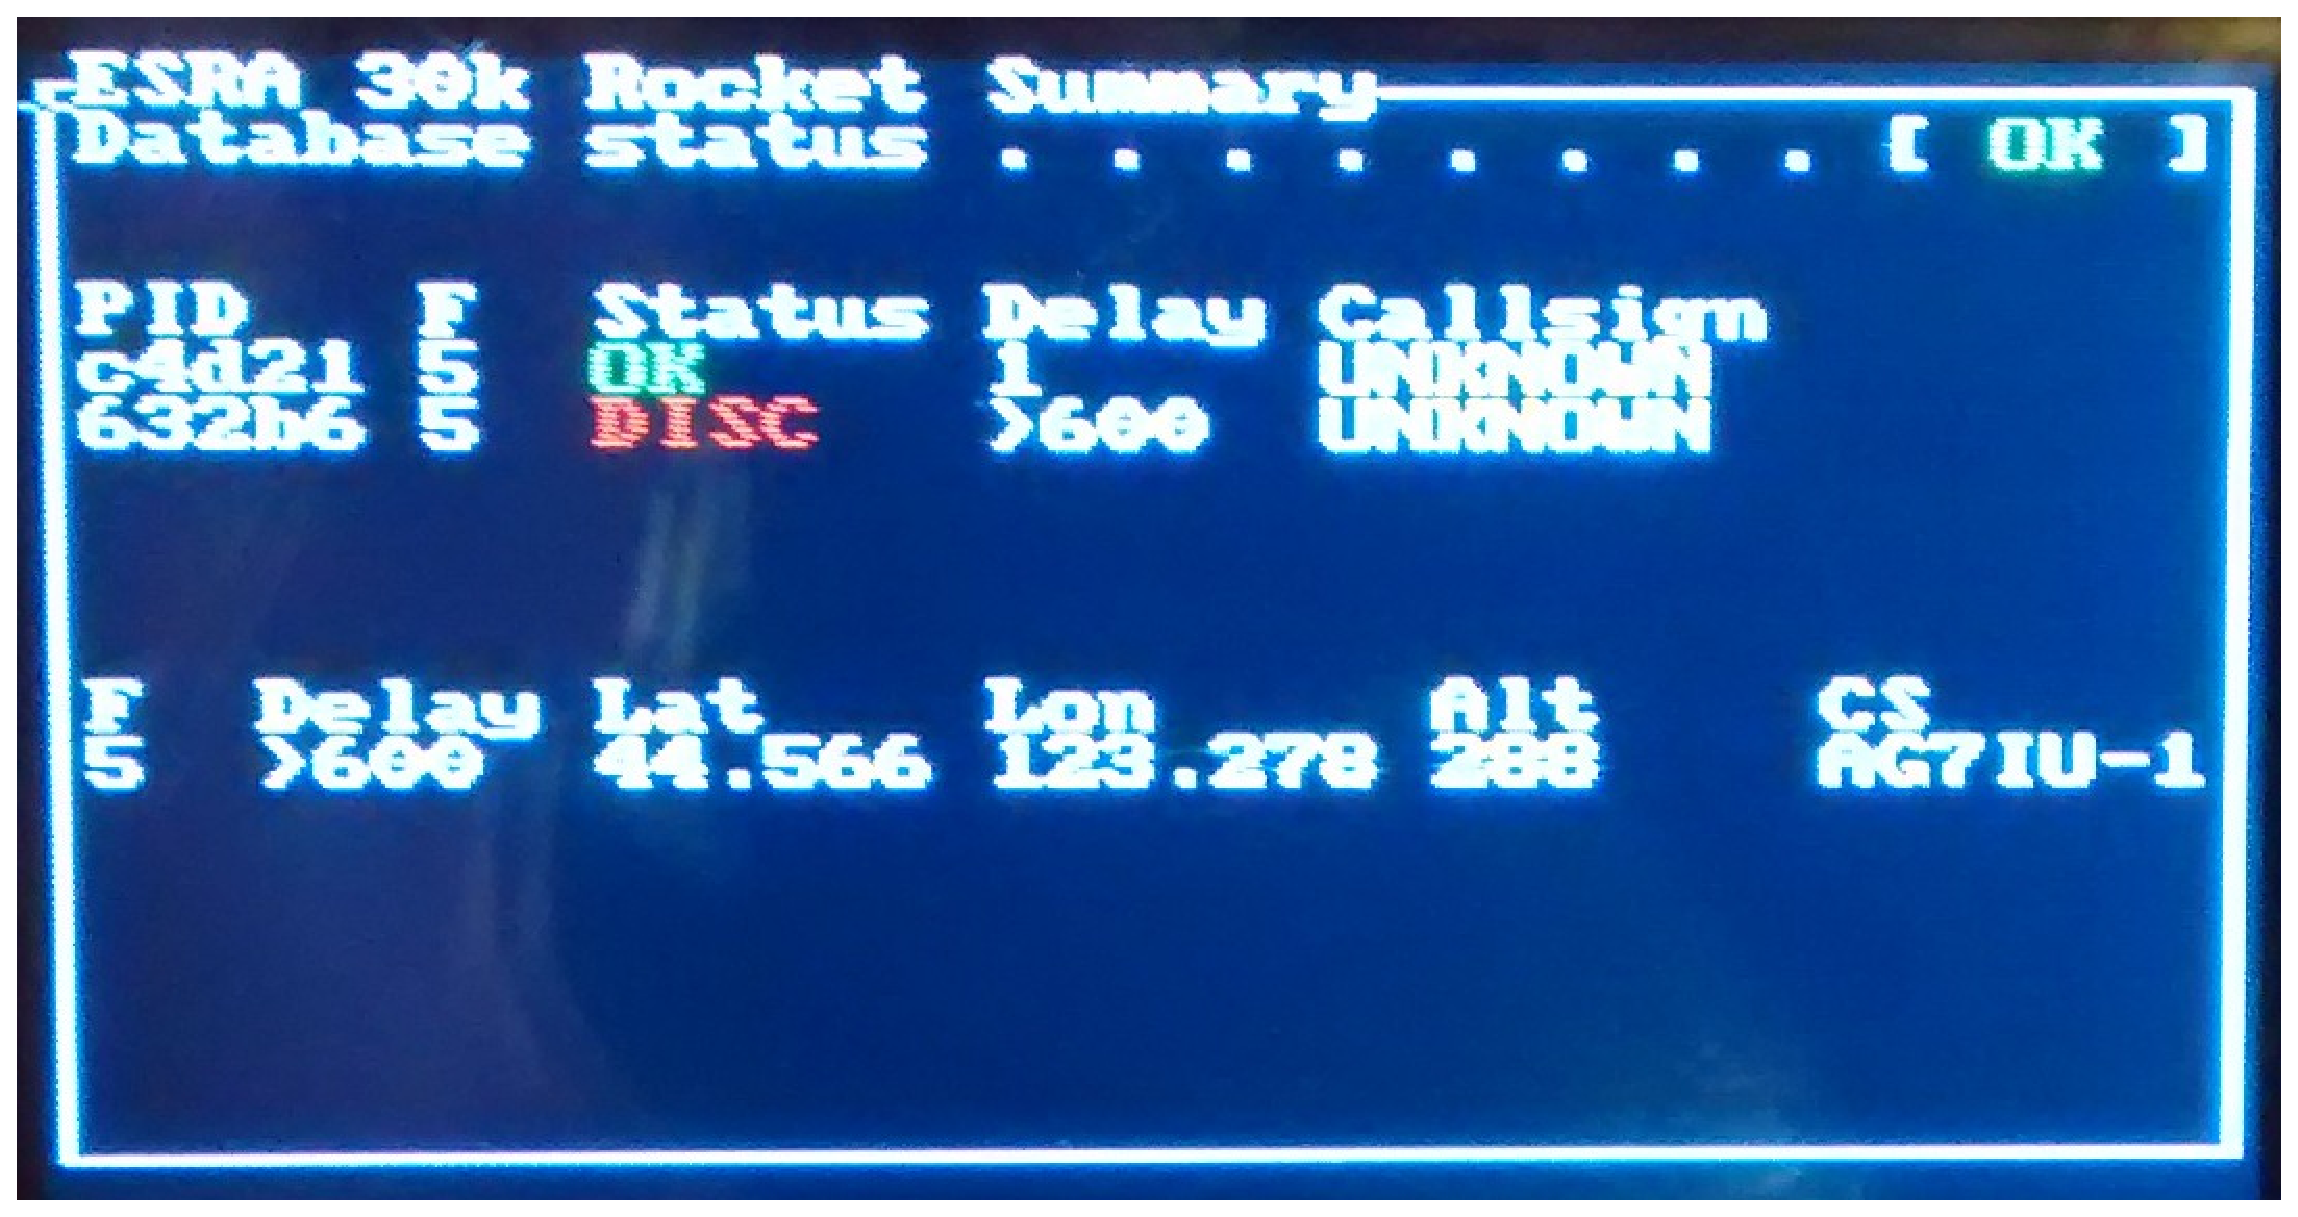
\includegraphics[width=.5\textwidth]{images/monitor.eps}
    \label{gs-monitor}
    \captionof{figure}{LCD in the ground station showing parser status and last location from the database.}
\end{center}

\subsubsection{Remaining Tasks}
The physical assembly has been a challenge for us.  We don't have the manufacturing tools and knowledge to reliably secure the components in way that is also visually appealing.  We assembled the ground station using plastic sheets and foam padding that are not ideal.

To solve this problem, we enlisted the help of a junior mechanical engineering student on the team, who is 3d printing a more visually impressive system to hold the computers and battery in place.  This is a good example of learning to work with our ESRA team members from different backgrounds, to create a better component than we could manufacture on our own.  If the 3d printed material does not work, our current version is made from bent and glued sheets of white plastic, which serve well enough.

The current ground station is effective and meets our goals, but we would like to make it look better.

%-------------------------------------------------------------------------------

\subsection{Networking}
Section by Allison Sladek

\subsubsection{Overview}
The Raspberry Pi 3B computer in the ground station will serve a local Wi-Fi network that nearby people can join to interact with our system. 
Each of the Raspberry Pi Zero computers will be networked to the main Pi 3B computer using USB OTG, which allows them to be powered and networked over a single USB cable.  
We will be able to ssh into the Pi 3B or Pi Zeros using this Wi-Fi network. 
This system should allow our teammates to connect to our web interface to view incoming flight data during the launches as well as any stored data from previous launches after it has been uploaded. 

\subsubsection{Current Progress}
The main Raspberry Pi 3B computer in the ground station has been configured to connect to any known Wi-Fi networks, or broadcast its own if there is none available. 
Nearby people can join this broadcasted network to test, program, or otherwise interact with our system. 
This system should allow our teammates to connect to our web interface to view incoming flight data during the launches as well as any stored data from previous launches after it has been uploaded.
This was done by editing configuration files on the Pi. 
This network has been sufficient for testing purposes, but a stress test during one of our weekly meetings revealed some issues that have yet to be addressed. 
Out of our group of about 25 people, about half of the room had some connectivity issues with our website. 

Each of the Raspberry Pi Zero computers are networked to the main Pi 3B computer using USB OTG, which allows them to be powered and networked over a single USB cable. The USB on-the-go connection was fairly straightforward to configure, and doesn’t currently have any known issues.


\subsubsection{Remaining Tasks}
A stress test from earlier in the project showed that we could support about a dozen users from the network hosted by the Raspberry Pi 3 in the ground station.
Our full team contains 18 students, plus several mentors.
Ideally the full team would be able to connect to the network at one time.
None of our requirements dealt with how many users we had to support with our web-based graph display site. 
However, if time allows, we may explore the possibility of adding a router to our ground station to allow more users to connect to our system. 
This change may improve our team's experience at the competition launch.
%-------------------------------------------------------------------------------
\subsection{Web Interface}
Section by Allison Sladek
\subsubsection{Overview}

Our goal for the web interface was to place the flight data graphs on a platform where they could be viewed by any of our team members. 
The flight viewer is meant to be accessible and to simplify the process of reviewing flight data after or during launches.

The entire website is divided up into handlebars partials to ensure that changes made in one section of the site carry over onto related elements without having copy and paste the same code into many different files. 
JQuery is also used pretty extensively for the purposes of retrieving and parsing JSON objects returned from database queries. 
The majority of elements on any one of the site's pages are populated from the database. Each of the drop downs on the navigation bar and the landing page run a query to add the appropriate flights available to display.

\subsubsection{Current Progress}
Over the course of the last two terms, the web interface has gone from a sketch on the back of a sheet of notebook paper to a fully functional graph viewing tool. The front end makes queries to the database housed on the same Raspberry Pi that hosts the web server and uses that data to populate graphs that update every second. Flights can be selected using either the drop down menus on the navigation bar or on the landing page. From a selected graph, the user can switch flights or graphs using the navigation bar, which will send a new query once a graph has been selected. This term, the website has gone through an aesthetic redesign, with a new dark theme and a layout that our team members will be familiar with.

\begin{center}
	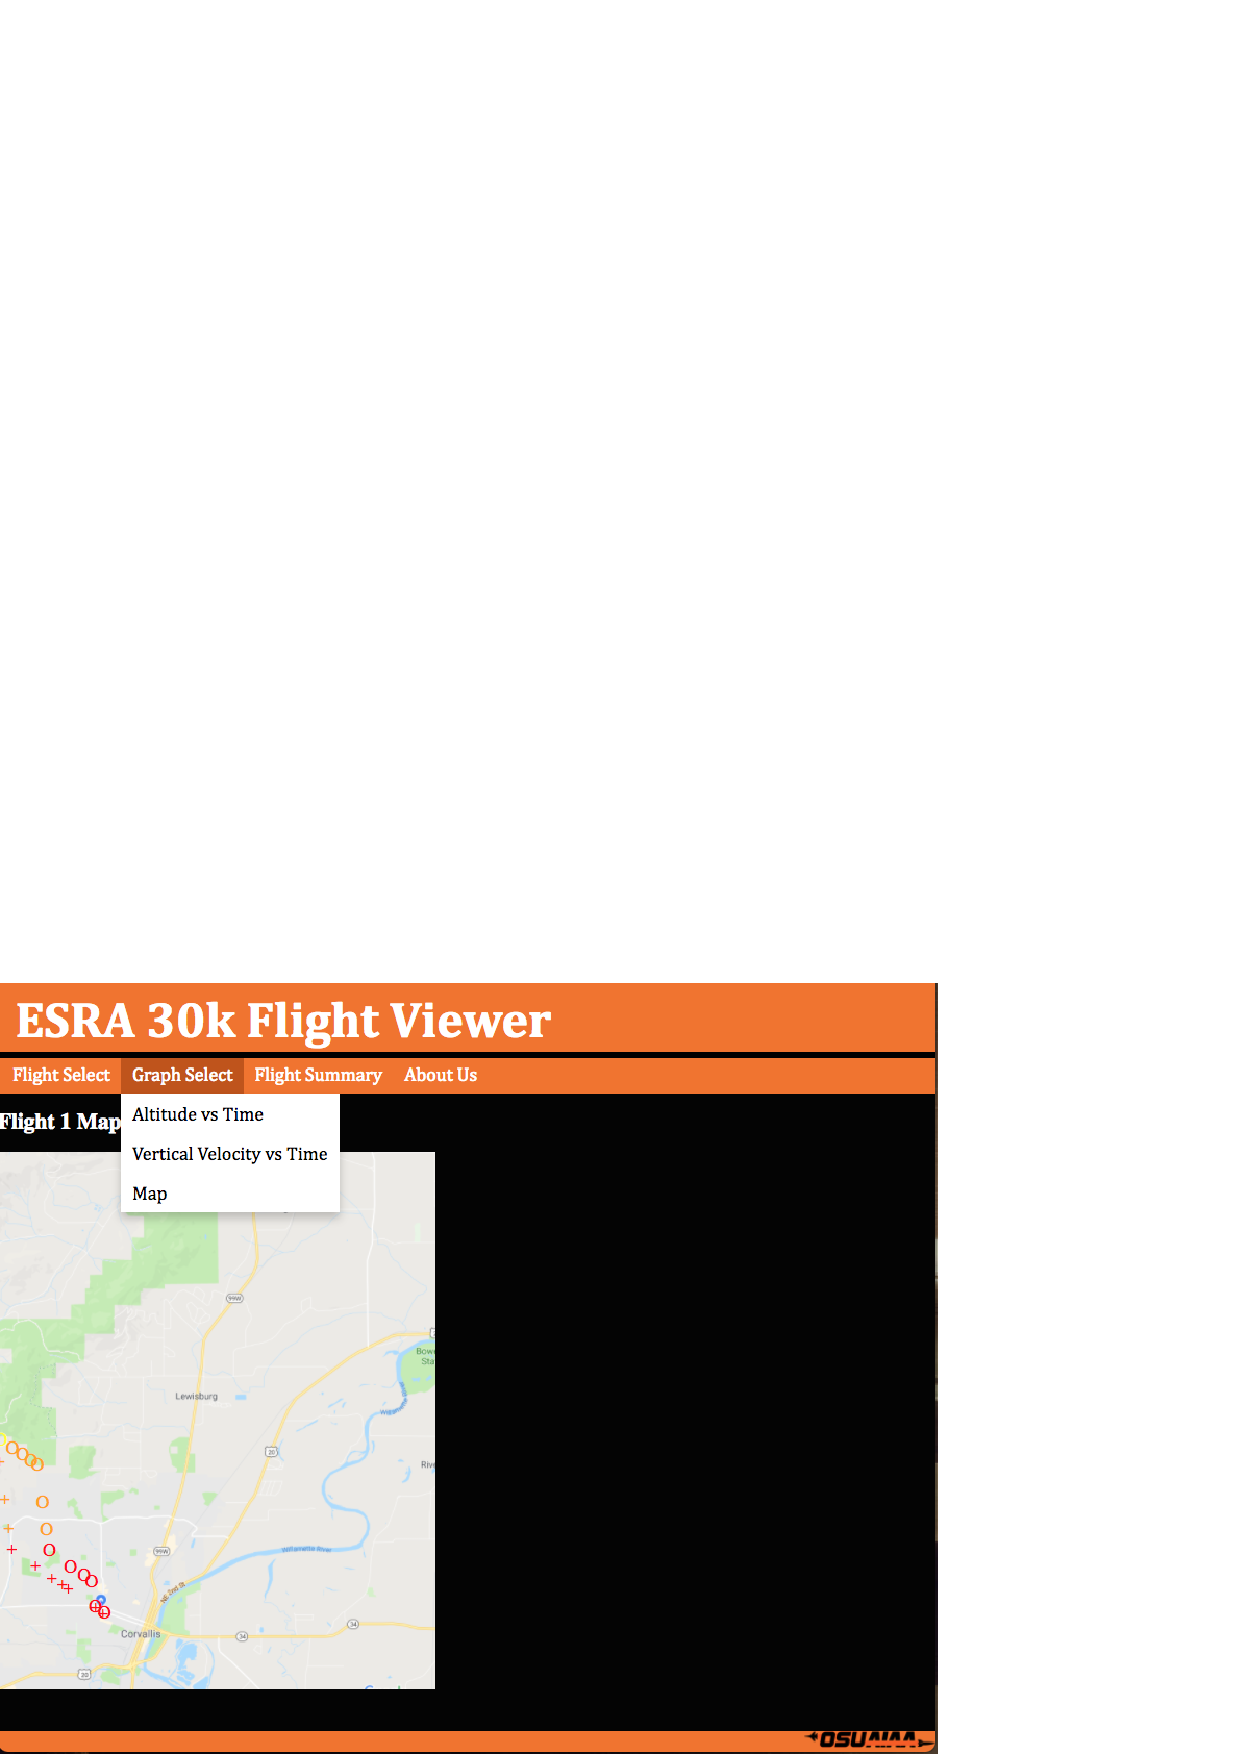
\includegraphics[width=0.5\textwidth]{images/smallMap.png}
    \label{gs-diagram}
    \captionof{figure}{Screenshot of the Flight Viewer}
\end{center}
       

%-------------------------------------------------------------------------------

\subsection{Graphs}
Section by Joshua Novak
\subsubsection{Overview}

Our goal is to create a readable display for the telemetry data received during and after flights. It should be able to display certain data within ten seconds of it being sent from the rocket, and should also be able to display data that has been uploaded to the database after a launch.
\subsubsection{Current Progress}

The Raspberry Pi 3B currently serves a web interface that users can connect to on mobile devices. This interface queries the database to receive new data at regular intervals, updating as new information is added to the database. Currently there are three plots, the altitude vs time plot, the vertical velocity vs time plot, and the gps coordinate plot. The altitude vs time plot is setup to receive input from up to six sources that correspond with a single flight ID, and plots the altitude of the rocket as recorded by that source vs the time it was recorded. The vertical velocity graph is similar, but instead displays the change in altitude, thus the specification of it being the vertical velocity. This is used instead of recorded velocity because we do not receive any recorded velocity mid-flight. Finally, the GPS coordinate map can plot the location of the rocket recorded by any source on a map. We use a saved map from google images for testing, and will do the same for the final map. We added a feature that displays the altitude and source of a point on the map when moused over, and that has the different sources come up as different characters. Finally, they also vary in color with altitude, making the map immensely more readable.

\subsubsection{Areas for Expansion}
It would be nice to setup graphs for acceleration or temperature, which may be useful for competition. We have uploaded implementations of these, but they have not yet been thoroughly tested. However, the queries and graphs are identical to those of altitude, so it will be easy to debug if it is not currently correct.

%-------------------------------------------------------------------------------

\subsection{Data Parser}
Section by Levi Willmeth
\subsubsection{Overview}
The parsing program takes an audio source for live telemetry data from a hand held radio on the same frequency as the telemetry transmitters in the rocket and payload.  The parsing program converts the audio signal into a string of text, validates the data using a checksum, separates the data into indidivual fields, and compares the data against expected fields.  Then it writes the data into a networked database.

A separate program allows us to import raw CSV files from either the rocket or payload avionics.  This feature was originally built into the parsing program, but we decided to separate it because the use cases are very different.  The parser program is intended to run headless and automatically, and the import program requires human interaction to determine which flight the CSV file should be associated with.  The parser program also requires additional libraries not necessary to import CSV files.  Therefore it made sense to separate these into two separate programs.

\subsubsection{Current Progress}
The current version of the data parser successfully runs simultaneously on four raspberry pi zeros in the ground station.  Each zero has a USB sound card and can process an audio signal from a single BeelineGPS telemetry unit on the rocket.  We have only had access to the actual telemetry parser one time, and only for a few minutes so far.  During this test the parser was able to successfully parse the radio signal and store data.  We have performed additional tests using recorded audio to simulate the radio signal.

The import program is able to import the latest CSV files from both the rocket and payload avionics.  The data is stored in the database.

To test the parser system, we have been using an audio file from the ECE's which includes progressively weaker signals because it was generated from a series of range tests up to 50 miles away.  We compared the performance of our parser against several other similar commercial products.  Our parser was able to decode 30/50 of the signals, compared to most commercial solutions decoding 30-31 and the absolute best commercial solution reportedly decoding 42/50.  We believe the difference comes from the quality of our inexpensive sound card vs a desktop PC dedicated sound card. We will continue to try to improve the performance, but based on our expected use case of ~10 miles, we are satisfied with our current results.

\subsubsection{Remaining Tasks}
As a stretch goal, we also want to be able to parse and store signals from the TeleMega telemtry unit, which includes many more data fields than the BeelineGPS.  These signals should be very similar to the actual payload files.  Instead of an audio signal, the TeleMega outputs serial data over USB, which should be readable from our parser program.

Due to frequent and unplanned (major changes as late as 4/24) modifications to the electronic hardware, we spent much of our development time refactoring avionics instead of implementing the TeleMega parser.  This was unfortunate but necessary, as the successful performance of the flight hardware takes precedence over a stretch goal that would only be used during the technology expo.

%-------------------------------------------------------------------------------

\subsection{Database}
Section by Levi Willmeth

\subsubsection{Overview}
The database is served by a Raspberry Pi 3B computer inside the ground station case.  The database collects and stores all data recorded during the flight, and relates records inserted at different times and from different sources by using a combination of primary and foreign keys. This will allow our web server to select records based on a given flight, or range of time, even though flight records are stored across several tables.

\subsubsection{Current Progress}
The database was one of the first components built.  It has undergone a few minor changes and updates to include fields for the latest electronics components, but the overall design has remained relatively stable.

Currently the BeelineGPS, Flights, Parser\_Status, and Payload\_Avionics tables are being actively used by our system, and are meeting our needs. We have been able to write all of the queries needed to insert telemetry and flight avionics data, as well as select that data to use in the display client.

\begin{center}
	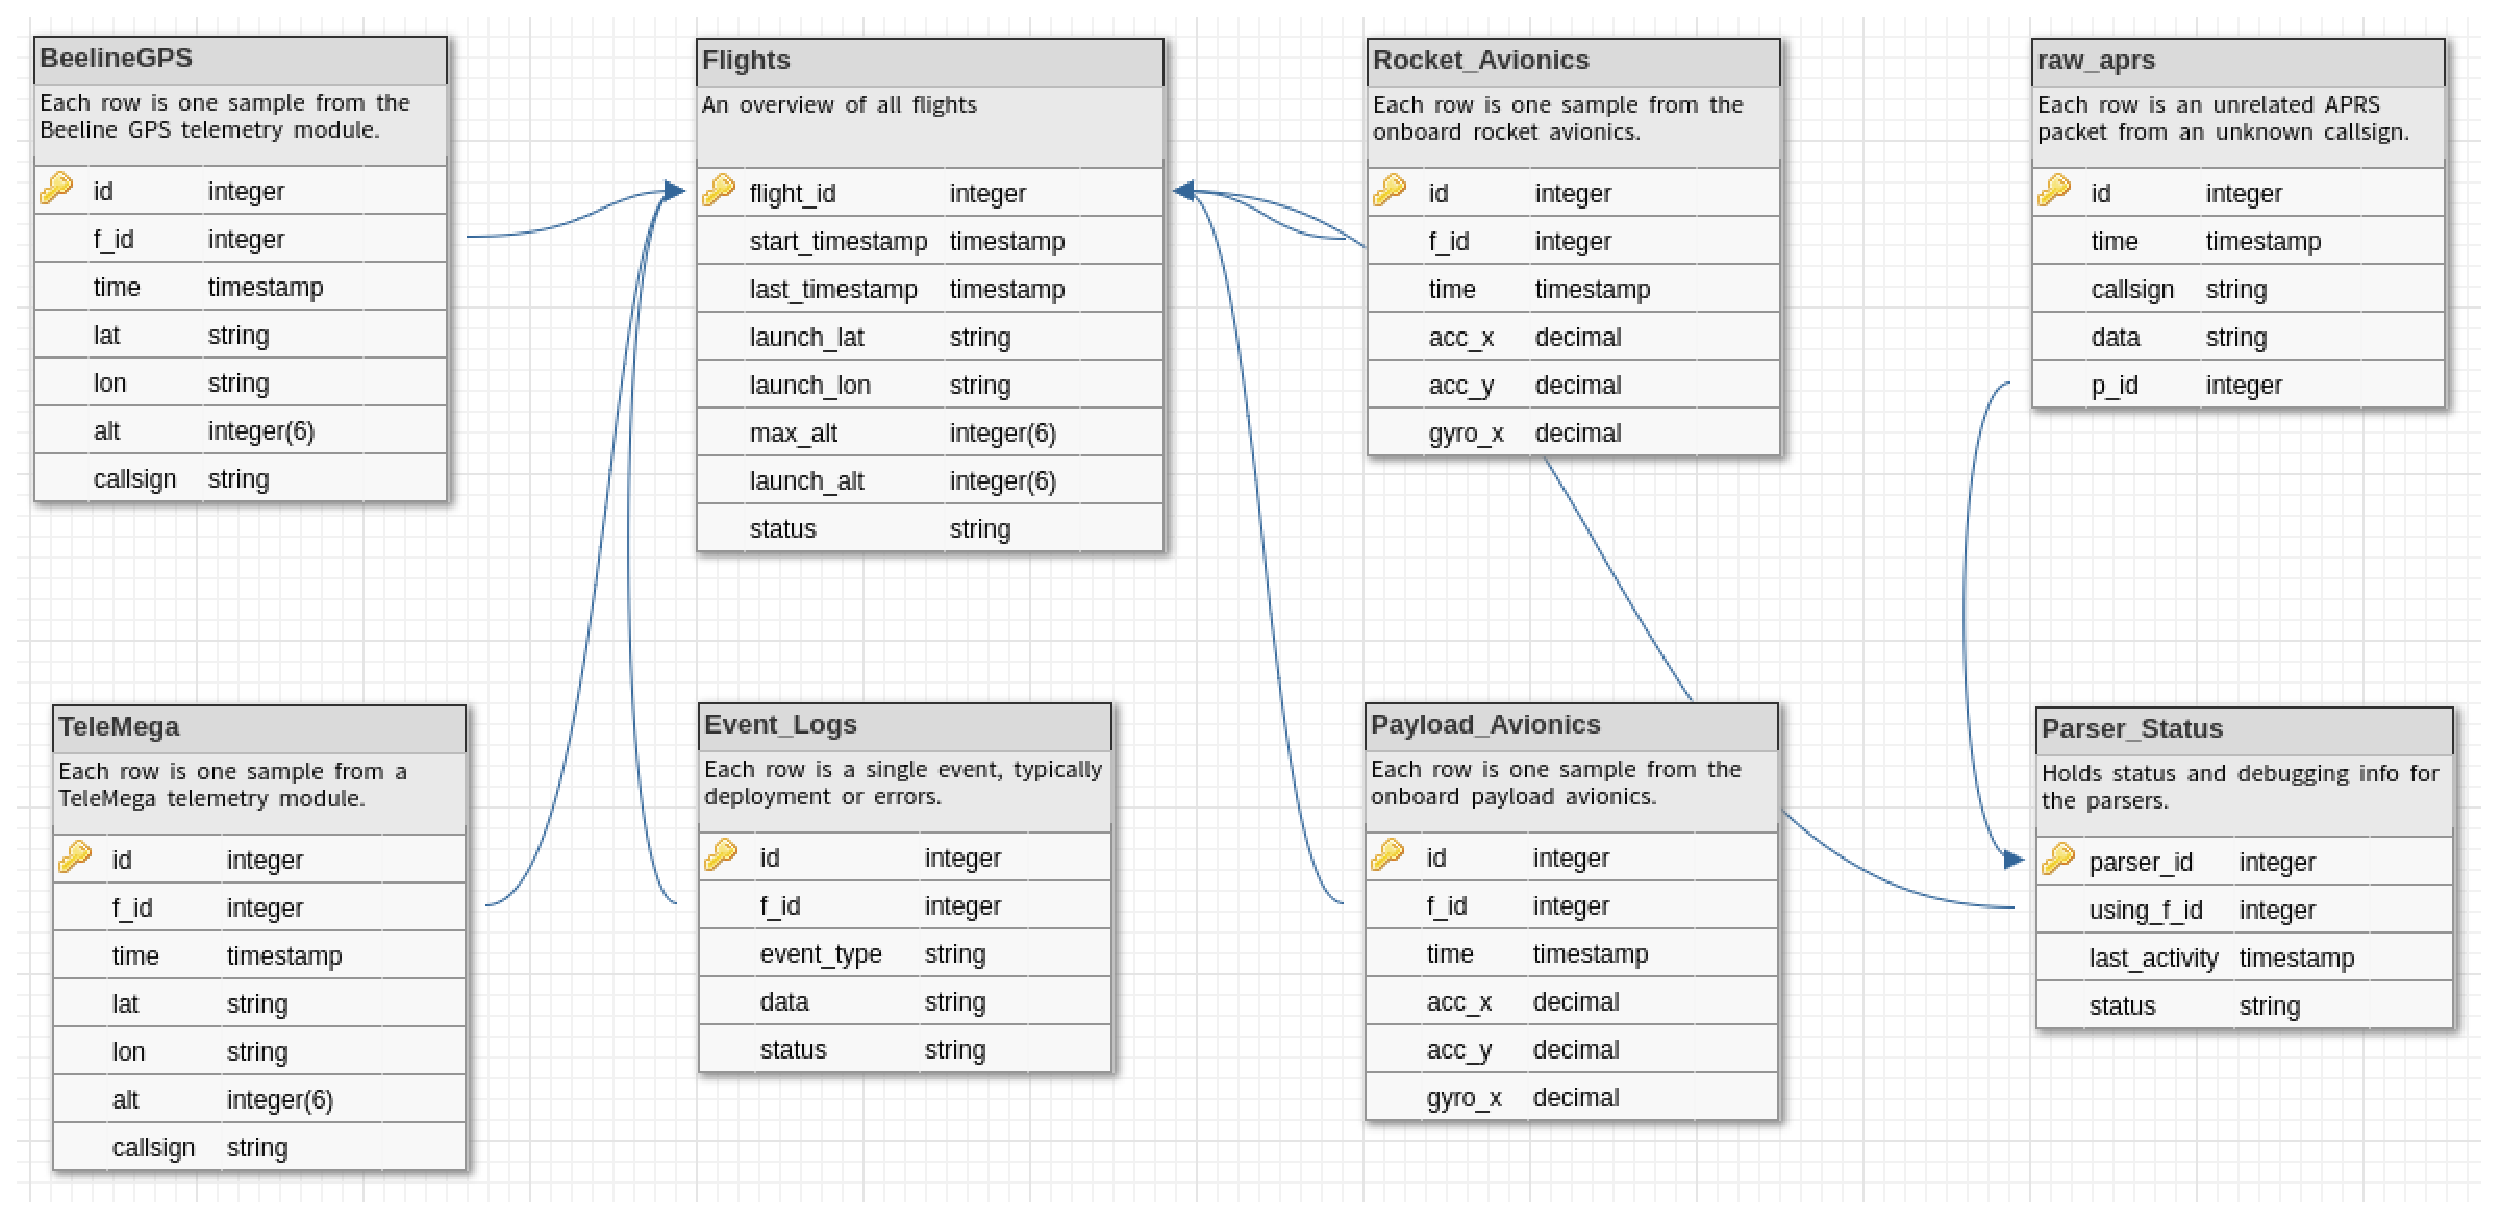
\includegraphics[width=.8\textwidth]{images/database_schema_v102.eps}
    \label{database-schema}
    \captionof{figure}{Current state of our database schema.}
\end{center}

\subsubsection{Remaining Tasks}
As the project continues we may find a need to update the database schema or make changes, but for now we consider the database to be finished.

%-------------------------------------------------------------------------------
\subsection{Sensor Avionics}
Section by Joshua Novak
\subsubsection{Overview}
For sensor avionics, the primary goal is to retrieve values from the different sensors installed on the rocket and format them into floats to be processed by the other avionics programs on the Raspberry Pi's. The sensors are connected to over an I2C bus.

\subsubsection{Current Progress}
Currently all of our sensors have been implemented and tested. Their reliability has been found to be quite high. We had planned on checking that they were within bounds, but found that the sensors themselves had very limited bounds for display that were lower than our expected limits (the accelerometers are parsed in such a manner they can only give values between -2 and 2, operating values for the thermometer are potential values for us to realistically encounter, etc), so this was found to be unnecessary. The exception was the altimeter, which can give large readings when it would go around to a negative value, and has a range of over five times our likely range, leading to a limit being put in place to filter out these potential issues. Most of the recent work on sensors has involved setting up ways to change the orientation of the accelerometer, speed up readings of the altimeter, and calibrate the accelerometer. All of these tasks have been completed. We have also added a method for offsetting the altimeter, which is similar to the method used by its own offset register.

\subsubsection{Areas for Expansion}
It may be necessary to add some kind of filter on values to reduce noise. We will know after our test launch.
%-------------------------------------------------------------------------------
\subsection{Rocket Avionics}
Section by Allison Sladek
\subsubsection{Overview}
The primary goals of the rocket avionics are to read and record values from the rocket sensors at a reasonable rate, ensure those stored values are recoverable after launch, and detect and record the moment of apogee. 
Many of these functions are similar to the functions of the payload avionics, so we may reuse code from each section for the other. 
The sensors have to be checked and recorded as quickly as is reasonable with the resources available.
More frequent samples will give more detailed data of the launch and allow better testing and analysis for post-launch. 
The values of the sensor data will be to be stored on the pi and made available after recovery of the rocket, or else no data will be revered from the launch, hindering our efforts of testing the rocket.
Apogee detection is very important to the success of the rocket. It normally triggers separation and parachute ejection, and without sensing it correctly, the rocket may deploy its parachute at the wrong time, or not at all. 

\subsubsection{Current Progress}
At the beginning of the project, it was stated that our rocket avionics would detect and trigger separation of the rocket, at apogee.  
Some time over winter, it was decided that the flight computer would not be connected to the separation charges.  
This decision was made by the ECE subteam without communicating with us.  As such, it will be impossible for us to trigger separation.
Instead, we will continue with our plan to detect apogee.  Instead of triggering separation, we will write a line to the log file.  That's as close as we can get to meeting our original goal of triggering separation.As much of the functions of the payload and rocket avionics overlap, there will likely be reused solutions between the two. 

Apogee detection is done through a state machine which performs checks with the flight sensors against threshold values to determine which stage of flight the rocket is in. The apogee event, when detected, transitions the rocket from the monitoring state to the descent state. 


\subsubsection{Remaining Tasks}
The threshold values in the state machine are based on values from others with similar apogee detection implementations, but we don't yet know that our rocket will see similar values while changing states. 
Each of our threshold values will have to be reviewed and tweaked after seeing the data from our upcoming first full test launch.


%-------------------------------------------------------------------------------

\subsection{Payload Avionics}
Section by Levi Willmeth

\subsubsection{Overview}
The Payload Avionics have three primary goals: use a propeller to push the payload towards the ground at the correct rate in order to neutralize gravity, to use a counterweight to reduce rotational momentum, to and record data from onboard sensors onto an SD card for later analysis.

The payload will be ejected from the body of the rocket at apogee, and attempt to create a zero gravity environment for 10-12 seconds during descent.  An array of sensors on the payload will rapidly measure the kinematics experienced by the payload.  A closed PID loop will use the latest acceleration values to calculate and control a pair of motors.  One motor will pull the payload downwards using a 10" propeller.  The second motor will spin a mass in the opposite direction to stabilize the rotation of the payload.  In this way, we hope to accelerate downwards at the same rate as gravity, to simulate stable spin and zero acceleration for 10-12 seconds.

Simultaneously, the payload will log sensor values onto an SD card in order to later analyze the performance of the payload and experiment.

\subsubsection{Current Progress}
Currently, the payload avionics are able to read from the current batch of sensors, which include three MPU9250 inertial measurement units for acceleration and rotation, a MPL3115A2 pressure sensor for altitude and temperature, and a PCF8523 real time clock for accurate timestamps.  It has been a difficult challenge to not have control over the sensors used because we needed to continually update our code whenever the components or wiring changed. Some of these changes occurred very late in the process, with the last major changes on April 17 and 24th of 2018.  We learned during the weekly meetings that our sensors had changed from a single MPU9250 to three MPU9250's, and that one of them would be rotated 180 degrees.  We had originally asked for three sensors but were told until now that it would be impossible due to limited space in the payload.

Despite this new challenge, we did our best and updated the payload avionics software to use the new sensor components, including accounting for the varied orientations.  This ended up quite challenging because our software was not designed for some sensors to be in different orientations.  We needed to remap each axis from the sensor onto a different axis in the avionics, including adjusting the sign.  In the end we were able to find a solution and are proud to say that our current version of the payload avionics software reads all of the flight sensors, uses a PID loop to calculate a motor speed based on the current acceleration, motor speed, and the time since last motor update.  It uses the acceleration calculation to drive the propeller's brushless motor via an attached ESC, and the rotational calculation to drive the DC motor and counterweight.

Finally, the avionics logs all of the sensor values to a text file in CSV format.  Because there are several sensors, and each sensor has several values, the current version of the avionics software generates a CSV file which has between 22-28 values per line (depending on flight stage), at a rate of about 90 lines per second (Hz).

We explored the idea of using a database on the payload because we thought it may be faster or more reliable.  Our tests showed that simply appending to a CSV file was about 20 Hz faster than using a database.  There may be table or algorithm optimizations to improve this scenario, but this was not a major aspect of the project and we could not justify the additional development time.

\subsubsection{Remaining Tasks}
We only received the actual flight hardware on 4/30/18 and initial tests showed several assembly problems including reversed SDA/SCL wires, shorted pins between the AD0 connections on all of the MPU's, and a 5v power supply to components requiring 3.3V.

We are working with the ECE team to troubleshoot these problems, but so far have not been able to complete a full end-to-end test of the payload system on the flight hardware.  We have successfully completed tests using our breadboard model using the agreed-upon pin configurations, but require working hardware from the ECE subteam to fully test the flight software on the actual flight hardware.

We will continue to work with the ECE team on this issue, and hope to have access to working hardware by our only practice launch on 5/12/18.

%-------------------------------------------------------------------------------
\subsection{Avionics Tests}
Section By Joshua Novak
\subsubsection{Overview}
The Avionics Tests are split into three categories, Unit Tests, which achieve code coverage to ensure code is functional and test that the code behaves as expected to expected inputs, hardware tests, which test how the code behaves when interacting with hardware such as motors or how it behaves during a launch, and simulation tests, which run a csv of inputs against the major logical decisions of the code.

\subsubsection{Current Progress}
In terms of Unit Tests, coverage has been achieved, though there is always room for improvement. There are also some aspects that are difficult to test using just unit tests, such as the motor controls and the like, as these need to be tuned based on how they affect the motors. Overall, I would say we have a solid test suite that one could continue building from were they to add more functionality to the code.

For hardware tests, we have mostly been waiting on getting our final hardware. We have recently been able to run our code on the ECE hardware, and have found that it runs effectively. We've also been able to run some code to spin motors, but not a full spin test with eveything loaded into the payload. We hope to complete that soon.

Finally, we have recently created a couple of simulation tools that check against the two state machines that were built for the rocket and payload respectively. They take a csv of important inputs as well as a factor for randomization and the sampling rate for the inputs. From this they run the inputs against the state machine, and output a csv with the randomized outputs and the state assigned to each input. This will allow for easy tuning of the state machine to fit the behavior of a likely flight, which will be important when transitioning from test launches to competition.

\subsubsection{Areas for Expansion}
There are always more tests that can be done, but most specifically it would be good to perform the spin test mentioned above and a test launch. Both are planned, but the launch has been delayed past code freeze while the spin test is waiting on several bits of hardware setup.
%-------------------------------------------------------------------------------

\section{Support the AIAA team as a whole}
\subsubsection{Overview}
One of our major goals for this project is to support the entire team, not just the computer science subteam.  To do our part, we have attended regular team meetings and do our best to understand the problems and challenges faced by the other subteams.  When have done our best to look for opportunities to help with tasks like component integration and rocket assembly.

\subsubsection{Current Progress}
As of the middle of Spring term, each of us have attended almost every team meeting.  On the rare occasion someone is unable to make it to a meeting, they have always been in contact with the other subteam members to let them know.

\subsubsection{Remaining Tasks}
This project is not over until the final competition in June, so we will continue to work together and grow as a team.

%===============================================================================

\end{document}
